\documentclass[hyperref=bookmarks]{beamer}

\usepackage{graphicx}
\usepackage{booktabs}
\usepackage[font=scriptsize]{caption}
\usepackage{fancybox}

% \usepackage[]{showframe}

\setbeamercovered{transparent}

\title{The Pope}
\author{Tejas Sanap}

\begin{document}
	% some stuff 
		\AtBeginSection[]
		{
			\begin{frame}
			\frametitle{Outline}
			\tableofcontents[currentsection]
			\end{frame}
		}

	\begin{frame}
		\maketitle
	\end{frame}

	\begin{frame}
		\frametitle{Outline}
		\tableofcontents
	\end{frame}
	
	\section{The Pope}
	\begin{frame}
		\frametitle{Who is the Pope?}

		\begin{columns}[T]
			\begin{column}{0.5\textwidth}
				The pope, also known as the supreme pontiff (pontifex maximus), is the bishop of Rome, leader of the worldwide Catholic Church, and head of state representing the Holy See. Since 1929, the pope has official residence in the Apostolic Palace in the Vatican City, the Holy See's city-state enclaved within Rome, Italy. The current pope is Francis, who was elected on 13 March 2013, succeeding Benedict XVI.
			\end{column}
			\begin{column}{0.4\textwidth}
				\begin{figure}[h!]
					\centering
					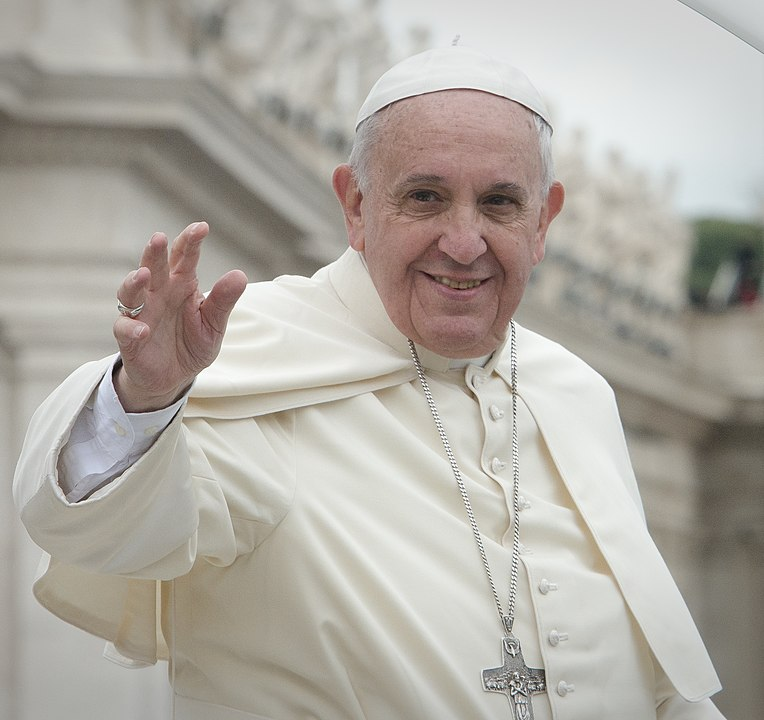
\includegraphics[width=\textwidth, keepaspectratio]{images/the-pope.jpg}
					\caption{Pope Francis}
					\label{img:the-pope}
				\end{figure}
			\end{column}
		\end{columns}
	\end{frame}

	\section{Previous Popes}
	\begin{frame}[fragile]
		\frametitle{Previous Popes}

		\begin{table}
			\centering
			\begin{tabular}{lccl}
				\toprule
				Name & YOB & YOD & Country \\
				\midrule
				Francis & 2013 & N/A & Argentina \\
				Benedict XVI & 2005 & 2013 & Germany \\
				John Paul II & 1978 & 2005 & Poland \\
				John Paul I & 1978 & 1978 & Italy \\
				\bottomrule
			\end{tabular}
			\caption{A list of previous Popes}
			\label{tab:the-popes1}
		\end{table}

		% \begin{minipage}{0.7\textwidth}
		% 	\begin{table}
		% 		\centering
		% 		\begin{tabular}{lccl}
		% 			\toprule
		% 			Name & YOB & YOD & Country \\
		% 			\midrule
		% 			Francis & 2013 & N/A & Argentina \\\uncover<2>
		% 			Benedict XVI & 2005 & 2013 & Germany \\\uncover<3>
		% 			John Paul II & 1978 & 2005 & Poland \\\uncover<4>
		% 			John Paul I & 1978 & 1978 & Italy \\\uncover<5>
		% 			\bottomrule
		% 		\end{tabular}
		% 		\caption{A list of previous Popes}
		% 		\label{tab:the-popes1}
		% 	\end{table}
		% \end{minipage}
		% \begin{minipage}{0.7\textwidth}
		% 	\begin{table}
		% 		\centering
		% 		\begin{tabular}{lccl}
		% 			\toprule
		% 			Name & YOB & YOD & Country \\
		% 			\midrule
		% 			Francis & 2013 & N/A & Argentina \\
		% 			Benedict XVI & 2005 & 2013 & Germany \\
		% 			John Paul II & 1978 & 2005 & Poland \\
		% 			John Paul I & 1978 & 1978 & Italy \\
		% 			\bottomrule
		% 		\end{tabular}
		% 		\caption{A list of previous Popes}
		% 		\label{tab:the-popes}
		% 	\end{table}
		% \end{minipage}
	\end{frame}

	\section{Blocks}
	\begin{frame}
		\frametitle{Blocks}
		\begin{block}{Triregnum}<1>
			Triregnum, also called the ``tiara". Recent popes have not, however, worn the triregnum, though it remains the symbol of the papacy and has not been abolished. In liturgical ceremonies the pope wears an episcopal mitre (an erect cloth hat).
		\end{block}
		\begin{block}{Crosier}<2-3>
			Crosier topped by a crucifix, a custom established before the 13th century.
		\end{block}
		\begin{alertblock}{WRONG!}<1-2>
			RUN!
		\end{alertblock}
		\begin{exampleblock}{Example?}<3->
			Example\ldots
		\end{exampleblock}
		\begin{block}{Some math}<4>
			$ a = a \times b $
		\end{block}
	\end{frame}

	\section{Various titles}
	\begin{frame}
		\frametitle{Various titles of the Pope}

		% \begin{itemize}
		% 		\pause
		% 	\item Bishop of Rome
		% 		\pause
		% 	\item Vicar of Jesus Christ
		% 		\pause
		% 	\item Successor of the Prince of the Apostles
		% 		\pause
		% 	\item Supreme Pontiff of the Universal Church
		% 		\pause
		% 	\item Primate of Italy
		% 		\pause
		% 	\item Archbishop and Metropolitan of the Roman Province
		% 		\pause
		% 	\item Sovereign of the Vatican City State
		% 		\pause
		% 	\item Servant of the servants of God
		% \end{itemize}

		% mess up the sequence
		% \begin{itemize}
		% 	\item<1> Bishop of Rome
		% 	\item<2> Vicar of Jesus Christ
		% 	\item<3> Successor of the Prince of the Apostles
		% 	\item<4> Supreme Pontiff of the Universal Church
		% 	\item<5> Primate of Italy
		% 	\item<6> Archbishop and Metropolitan of the Roman Province
		% 	\item<7> Sovereign of the Vatican City State
		% 	\item<8> Servant of the servants of God
		% \end{itemize}
		
		% \item<1-> Bishop of Rome
		% \begin{itemize}[<+->]

		% \begin{itemize}
		% 	\item Bishop of Rome
		% 	\item Vicar of Jesus Christ
		% 	\item Successor of the Prince of the Apostles
		% 	\item Supreme Pontiff of the Universal Church
		% 	\item Primate of Italy
		% 	\item Archbishop and Metropolitan of the Roman Province
		% 	\item Sovereign of the Vatican City State
		% 	\item Servant of the servants of God
		% \end{itemize}

		\begin{itemize}
			\item Bishop of Rome
			\item Vicar of Jesus Christ
			\item Successor of the Prince of the Apostles
			\item Supreme Pontiff of the Universal Church
			\item Primate of Italy
			\item Archbishop and Metropolitan of the Roman Province
			\item Sovereign of the Vatican City State
			\item Servant of the servants of God
		\end{itemize}
	\end{frame}

	\section{Overlay - onslide}
	% + makes something transparent
	% * makes something invisible
	\begin{frame}
		\frametitle{ONSLIDE - Some things the pope has said.}

		\onslide<1->{The unjust distribution of goods persists, creating a situation of social sin that cries out to Heaven and limits the possibilities of a fuller life for so many of our brothers.}
		\onslide<4->{Human rights are not only violated by terrorism, repression or assassination, but also by unfair economic structures that creates huge inequalities.}
		\onslide<3->{This is what I want, a poor Church for the poor.}
		\onslide<2->{I say that politics is the most important of the civil activities and has its own field of action, which is not that of religion.}
	\end{frame}

	\section{Overlay - uncover} 
	\begin{frame}
		\frametitle{UNCOVER - Some things the pope has said II.}

		\uncover<1->{The unjust distribution of goods persists, creating a situation of social sin that cries out to Heaven and limits the possibilities of a fuller life for so many of our brothers.}
		\uncover<2->{Human rights are not only violated by terrorism, repression or assassination, but also by unfair economic structures that creates huge inequalities.}
		\uncover<3->{This is what I want, a poor Church for the poor.}
		\uncover<4->{I say that politics is the most important of the civil activities and has its own field of action, which is not that of religion.}
	\end{frame}

	\section{Overlay - only} 
	\begin{frame}
		\frametitle{ONLY - Some things the pope has said III.}

		\only<1->{The unjust distribution of goods persists, creating a situation of social sin that cries out to Heaven and limits the possibilities of a fuller life for so many of our brothers.}
		\only<4->{Human rights are not only violated by terrorism, repression or assassination, but also by unfair economic structures that creates huge inequalities.}
		\only<3->{This is what I want, a poor Church for the poor.}
		\only<2->{I say that politics is the most important of the civil activities and has its own field of action, which is not that of religion.}
	\end{frame}

	\section{Overlay - visible}
	\begin{frame}
		\frametitle{VISIBLE - Some things the pope has said IV.}

		\visible<1->{The unjust distribution of goods persists, creating a situation of social sin that cries out to Heaven and limits the possibilities of a fuller life for so many of our brothers.}
		\visible<4->{Human rights are not only violated by terrorism, repression or assassination, but also by unfair economic structures that creates huge inequalities.}
		\visible<3->{This is what I want, a poor Church for the poor.}
		\visible<2->{I say that politics is the most important of the civil activities and has its own field of action, which is not that of religion.}
	\end{frame}

	\section{Overlay - invisible}
	\begin{frame}
		\frametitle{INVISIBLE - Some things the pope has said IV.}

		\invisible<1->{The unjust distribution of goods persists, creating a situation of social sin that cries out to Heaven and limits the possibilities of a fuller life for so many of our brothers.}
		\invisible<4->{Human rights are not only violated by terrorism, repression or assassination, but also by unfair economic structures that creates huge inequalities.}
		\invisible<3->{This is what I want, a poor Church for the poor.}
		\invisible<2->{I say that politics is the most important of the civil activities and has its own field of action, which is not that of religion.}
	\end{frame}

	\begin{frame}
		\centering
		\fbox{\fontsize{42.99}{48} \selectfont Thank You!}
		\vskip1\baselineskip
		\shadowbox{\fontsize{42.99}{48} \selectfont Thank You!}
		\vskip1\baselineskip
		\Ovalbox{\fontsize{42.99}{48} \selectfont Thank You!}
	\end{frame}

\end{document}
